\section{Durchf\"{u}hrung}

Zur Messung der Gitterschwingungen wird ein pump-probe-Aufbau verwendet. Die durch die Oszillation der Gitterschwingungen hervorgerufene, periodische Reflektivitätsänderung wird bestimmt, indem die Intensität des von der Probe reflektierten probe-Laserstrahls mit einer Photodiode gemessen wird. Dazu wird der in \autoref{aufbau} schematisch dargestellte Aufbau zunächst einjustiert. Sowohl der pump-Laser mit einer Wellenlänge von \SI{1047}{\nano\metre} und einem Fokus von \SI{20}{\micro\metre}, als auch der probe-Laser mit einer Wellenlänge von \SI{780}{\nano\metre} und einem Fokus von \SI{2}{\micro\metre} müssen auf die gleiche Stelle auf der Probe gerichtet sein. Das reflektierte Licht muss weiterhin auf die beiden Photodioden treffen.\par
Als erstes wird der Film ohne Höhenprofil angeregt und die Reflektivität gemessen. Daraus wird die Energiedissipation im Galfenol-Film bestimmt. Diese Messung wird im Folgenden von allen weiteren Messungen als Untergrund subtrahiert. Es werden vier Gitter unterschiedlicher Tiefe vermessen und für das tiefste Gitter außerdem die Polarisation gedreht. Aus der Intensität wird die Oszillation der Reflektivitätsänderung der Probe bestimmt. Mit einer Fouriertransformation der Messwerte in der Zeitdomäne lassen sich Amplitude, Frequenz und Breite des Signals untersuchen.
\begin{figure}
  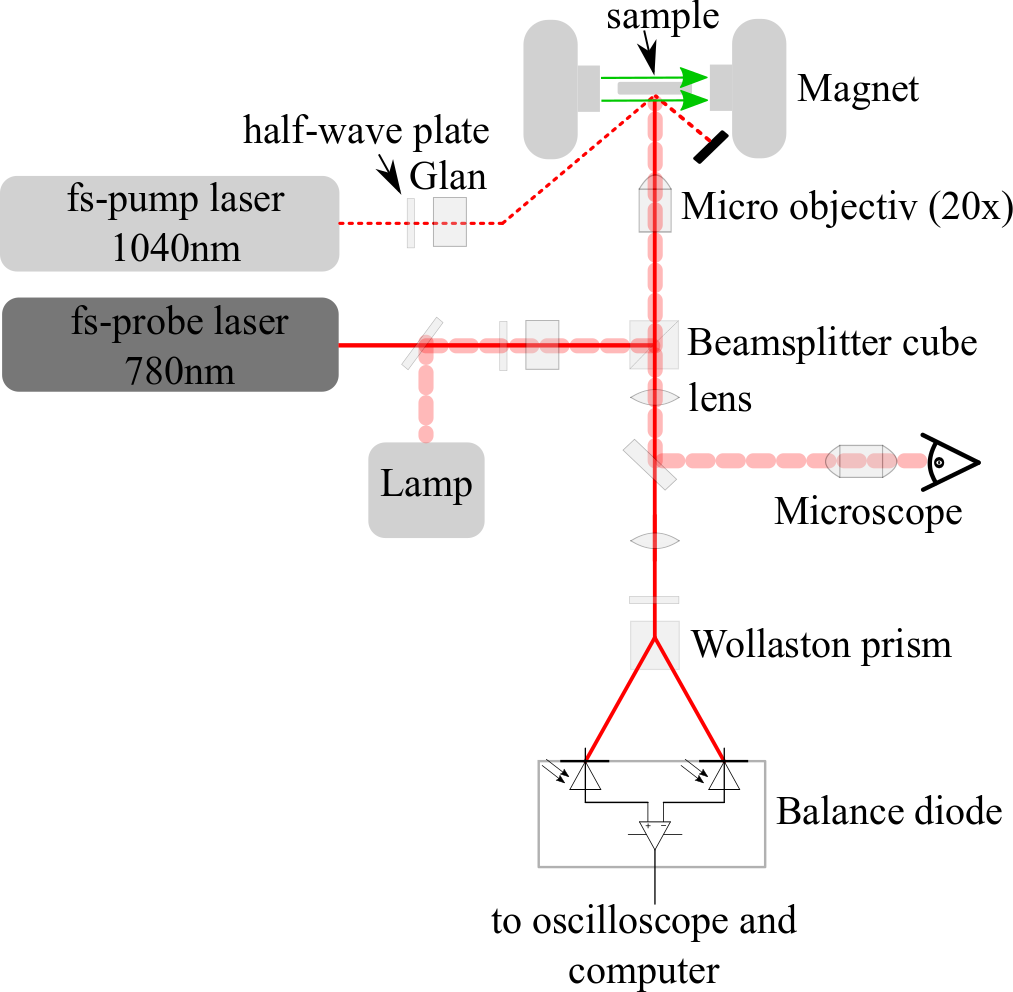
\includegraphics[width=\textwidth]{img/aufbau.png}
  \caption{Schematischer Aufbau der Messapparatur \cite{FP}}
  \label{aufbau}
\end{figure}

\FloatBarrier
